%%%%%%%%%%%%%%%%%%%%%%%%%%%%%%%%%%%%%%%%%%%%%%%%%%%%%%%%%%%%%%%%%%%%%%%%%%%%%%%%%%
%%% Navigation
%%% 
%%%
%%%%%%%%%%%%%%%%%%%%%%%%%%%%%%%%%%%%%%%%%%%%%%%%%%%%%%%%%%%%%%%%%%%%%%%%%%%%%%%%%%
\chapter{Navigation Results} \label{ch:results_navigation}

% The structure of this chapter needs revision.

% What do we have to talk about here?
% Well, I suppose the point of this chapter is to present how well the algorithm worked.
% What is there to present?
% I suppose it should be shown that the algorithm does indeed nav the robot,
% as that is not necessarily assumed in the chapter explaining the navigation.
% Some things you might want to know:
% Qualitatively, how well did it nav the robot?

% Ok, so what can I show?
% I can show pictures of the Nao naving around different environments getting to goals
% I can show what the robot thought his pose was based on the goal.
% I can list the optimal parameters for naving.
% I wish I could have shown laser data, because maybe I could have shown a potential field map.
% Can I show the different parts of what the nav was using? No, because the straight line planner
% and escape strategy was not implemented.

Shit. Now I have a bunch of plots that I need to say things about.

WHAT ARE THE OPTIMAL PARAMETERS/PARAMETERS USED.

\begin{figure}
  \centerline{
    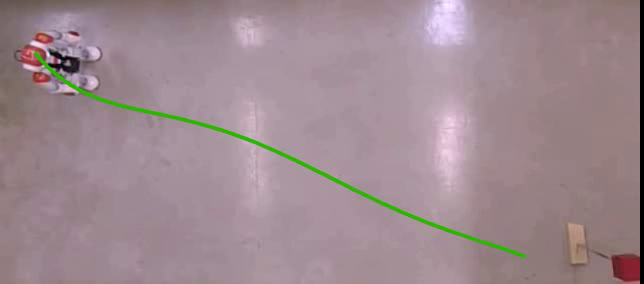
\includegraphics[width=0.5\textwidth]{nav/open/path/open_path1.png}
    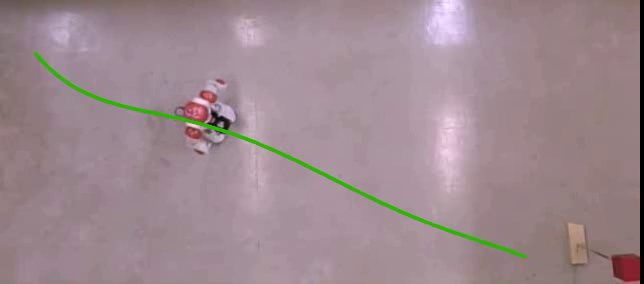
\includegraphics[width=0.5\textwidth]{nav/open/path/open_path2.png}
  }
  \vspace*{0.05in}
  \centerline{
    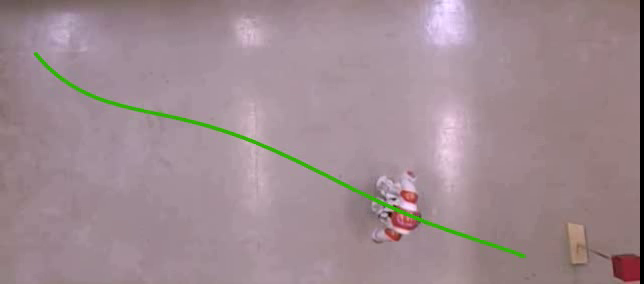
\includegraphics[width=0.5\textwidth]{nav/open/path/open_path3.png}
    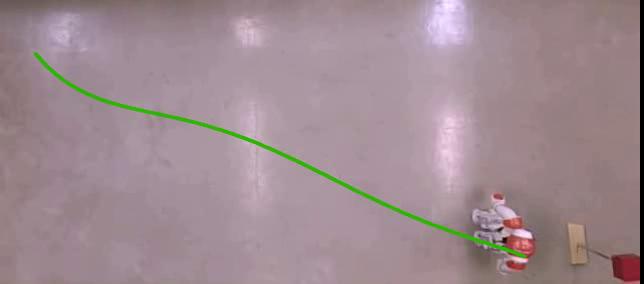
\includegraphics[width=0.5\textwidth]{nav/open/path/open_path4.png}
  }
  \caption{The periodic sequence of motion segments and robot postures in the proposed low-profile crawling gait. A 6-inch marker is shown in the background as a length scale reference.}
  \label{fig:nav_open_frames1}
  \vspace*{-0.07in}
\end{figure}

\begin{figure}
  \centerline{
    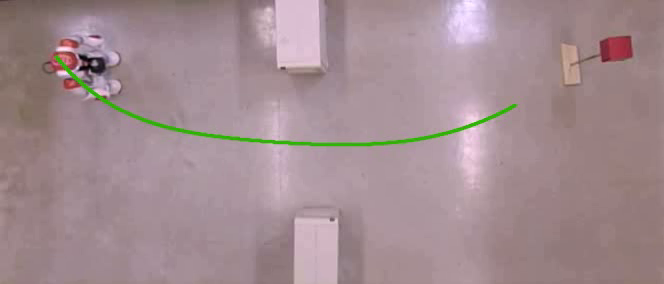
\includegraphics[width=0.5\textwidth]{nav/narrow/path/narrow_path1.png}
    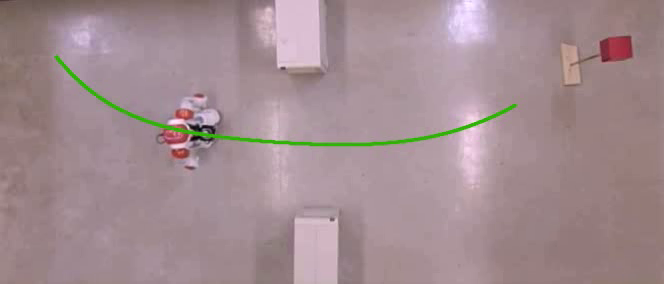
\includegraphics[width=0.5\textwidth]{nav/narrow/path/narrow_path2.png}
  }
  \vspace*{0.05in}
  \centerline{
    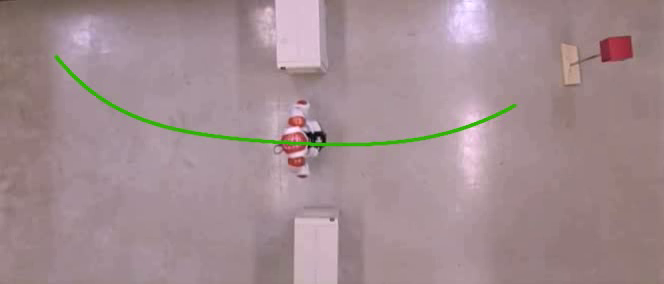
\includegraphics[width=0.5\textwidth]{nav/narrow/path/narrow_path3.png}
    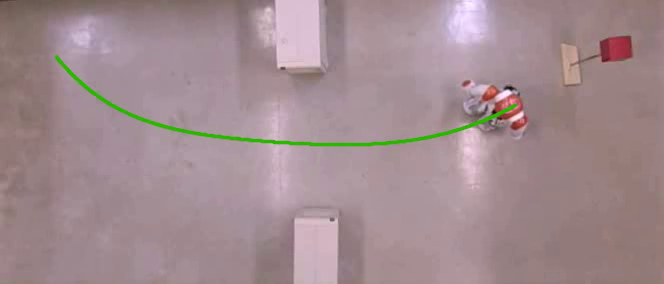
\includegraphics[width=0.5\textwidth]{nav/narrow/path/narrow_path4.png}
  }
    \caption{The periodic sequence of motion segments and robot postures in the proposed low-profile crawling gait. A 6-inch marker is shown in the background as a length scale reference.}
    \label{fig:nav_narrow_frames1}
        \vspace*{-0.07in}
\end{figure}

\begin{figure}
  \centerline{
    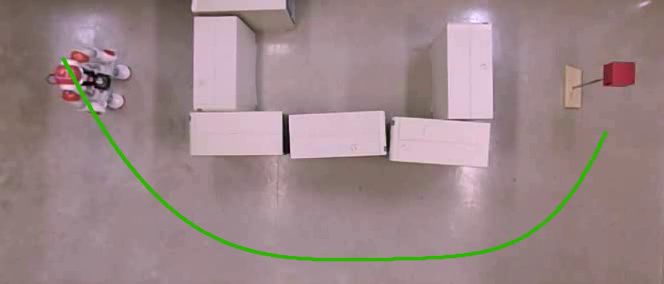
\includegraphics[width=0.5\textwidth]{nav/square/path/square_path1.png}
    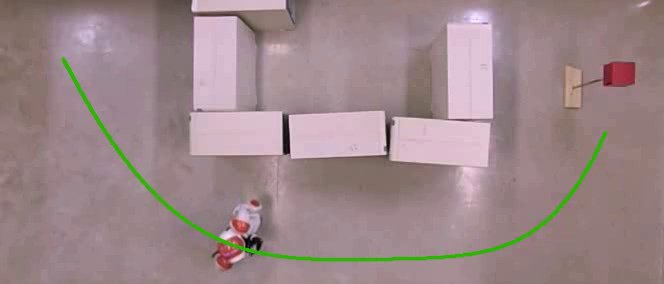
\includegraphics[width=0.5\textwidth]{nav/square/path/square_path2.png}
  }
  \vspace*{0.05in}
  \centerline{
    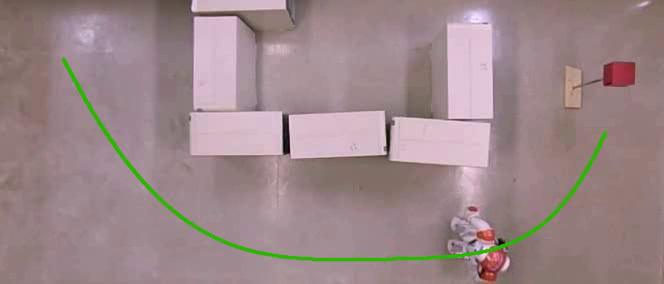
\includegraphics[width=0.5\textwidth]{nav/square/path/square_path3.png}
    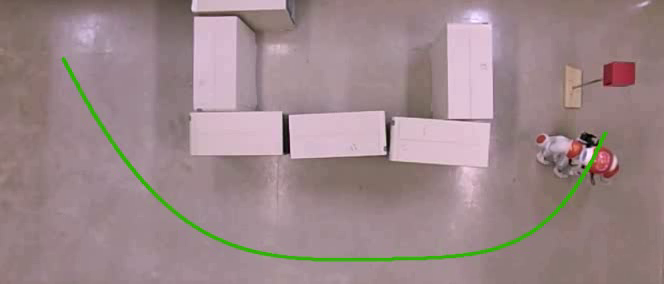
\includegraphics[width=0.5\textwidth]{nav/square/path/square_path4.png}
  }
    \caption{The periodic sequence of motion segments and robot postures in the proposed low-profile crawling gait. A 6-inch marker is shown in the background as a length scale reference.}
    \label{fig:nav_square_frames1}
        \vspace*{-0.07in}
\end{figure}

\begin{figure}
  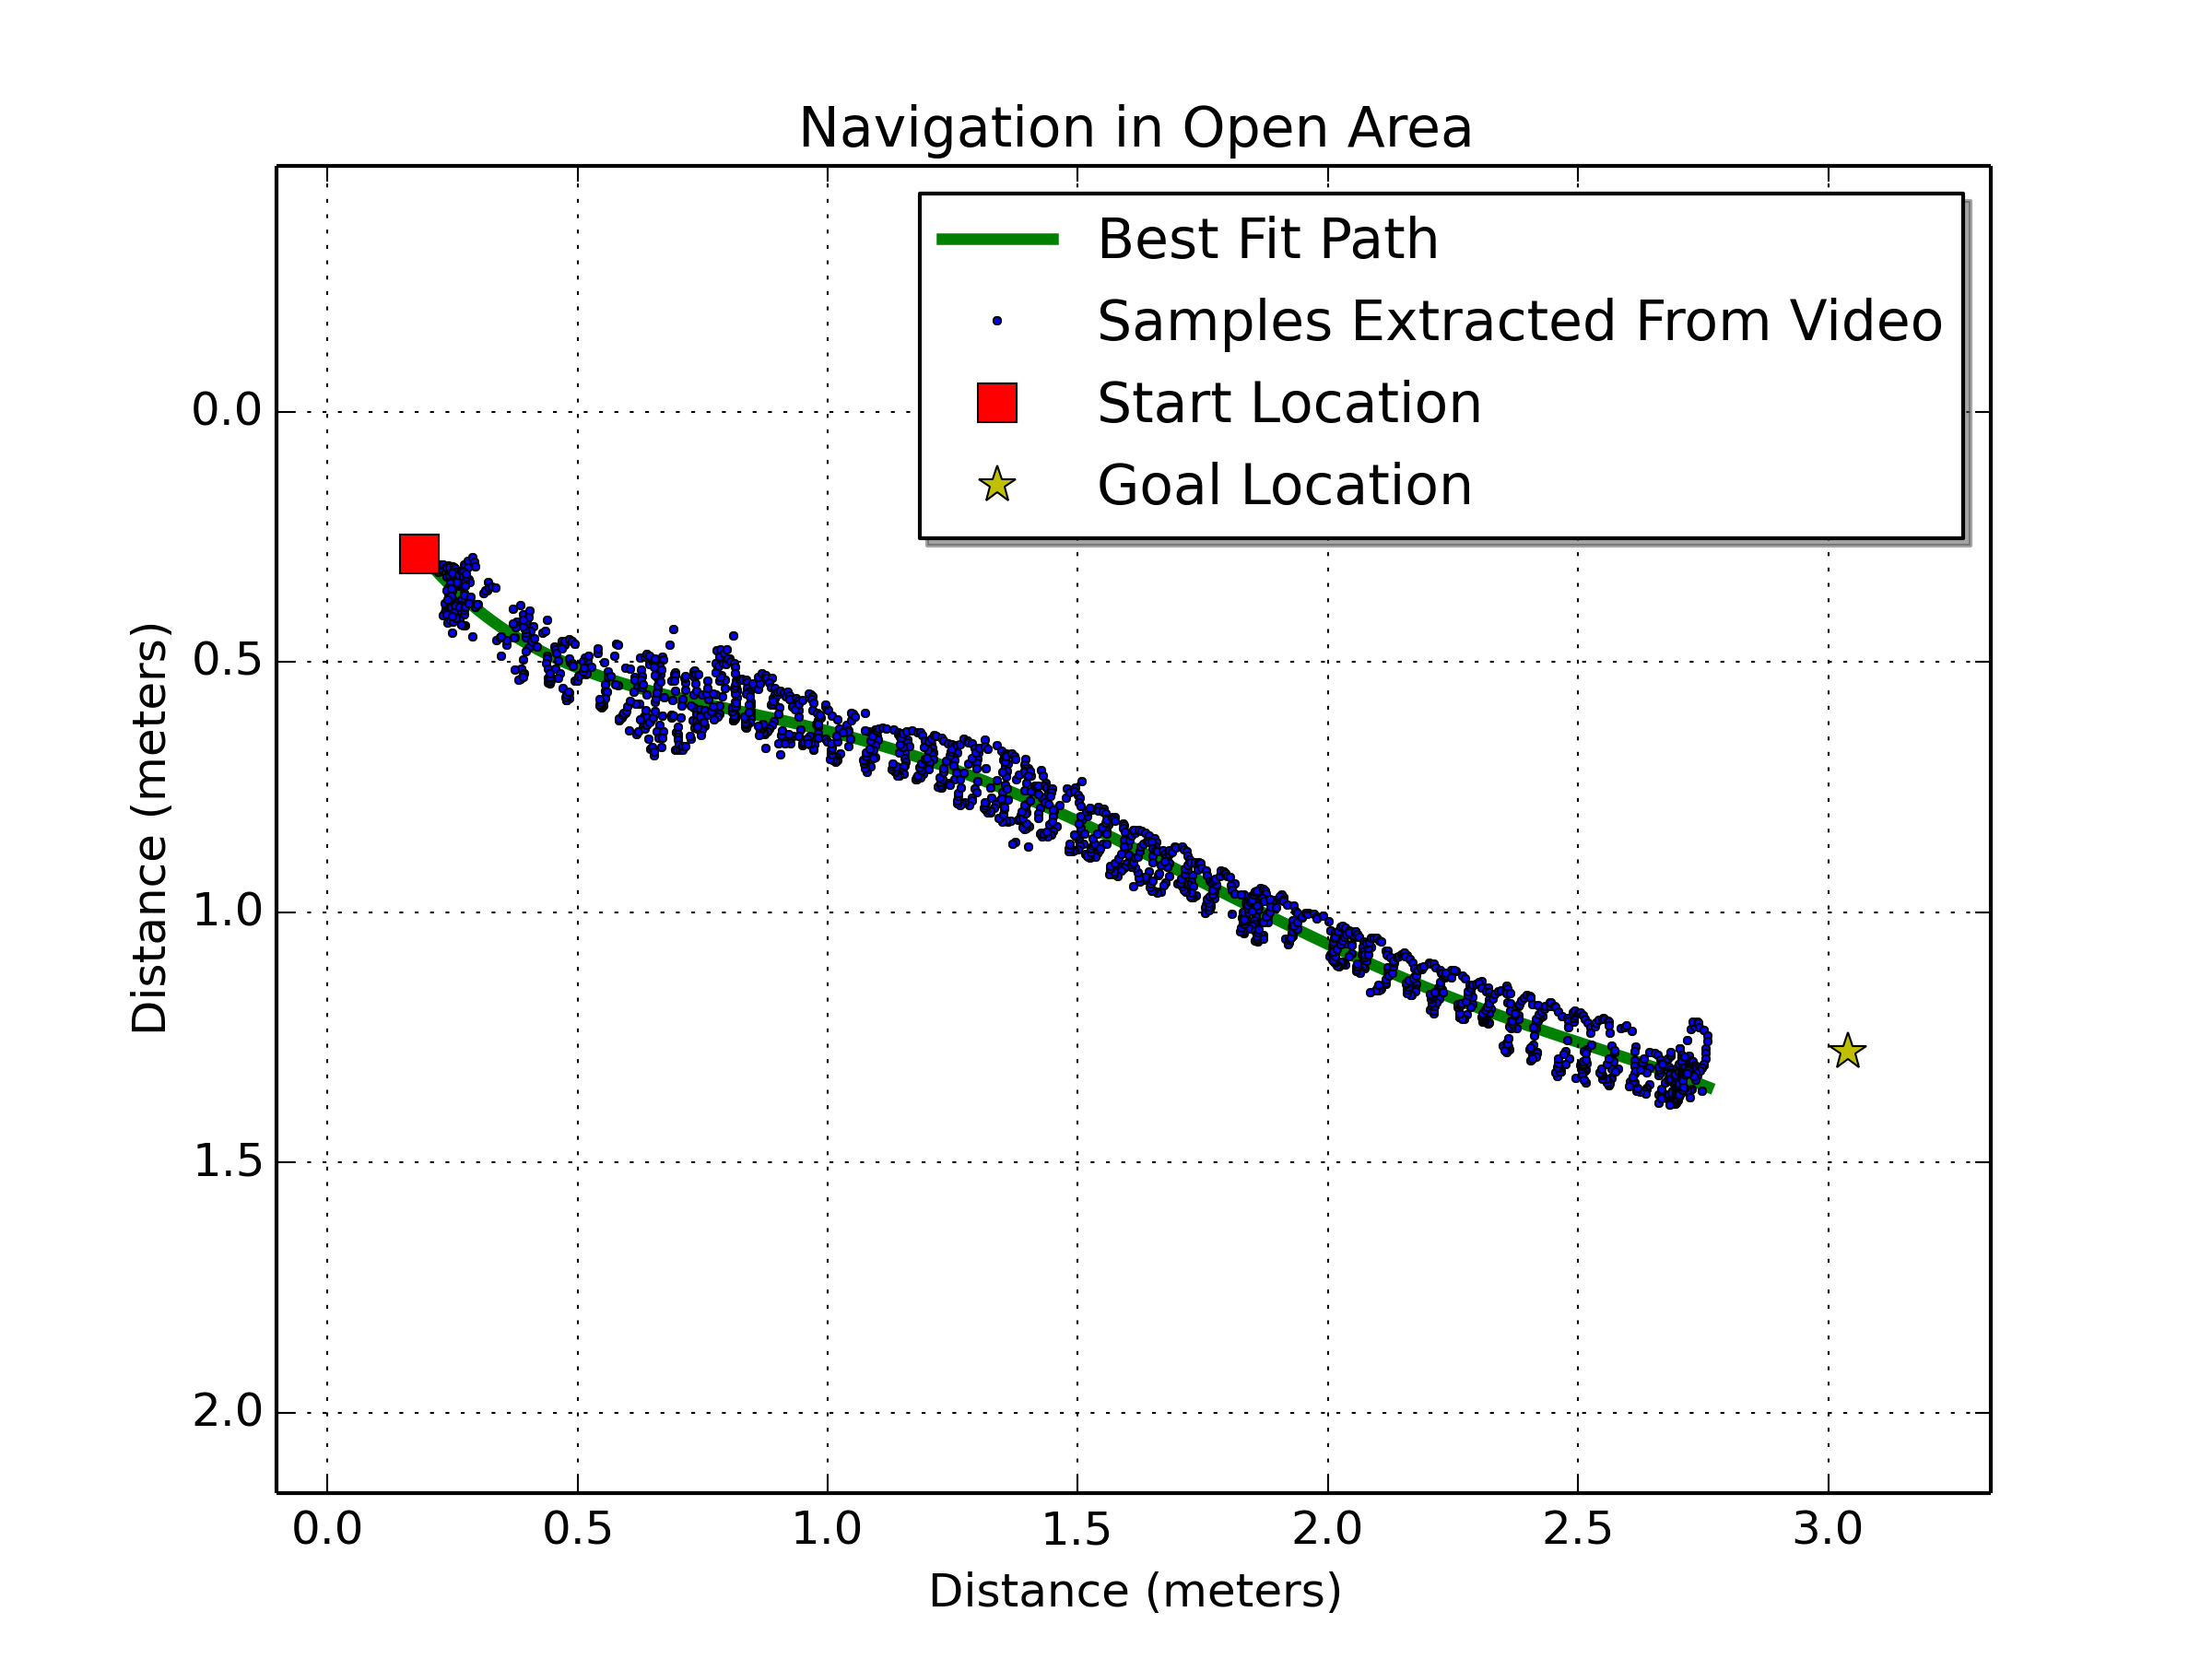
\includegraphics[width=\textwidth]{nav/open/plots/nav_open.png}
  \caption{Low-profile crawling gait for accessing vertically constrained spaces such as under a table.}
  \label{fig:nav_open_plot1}
\end{figure}

\begin{figure}
  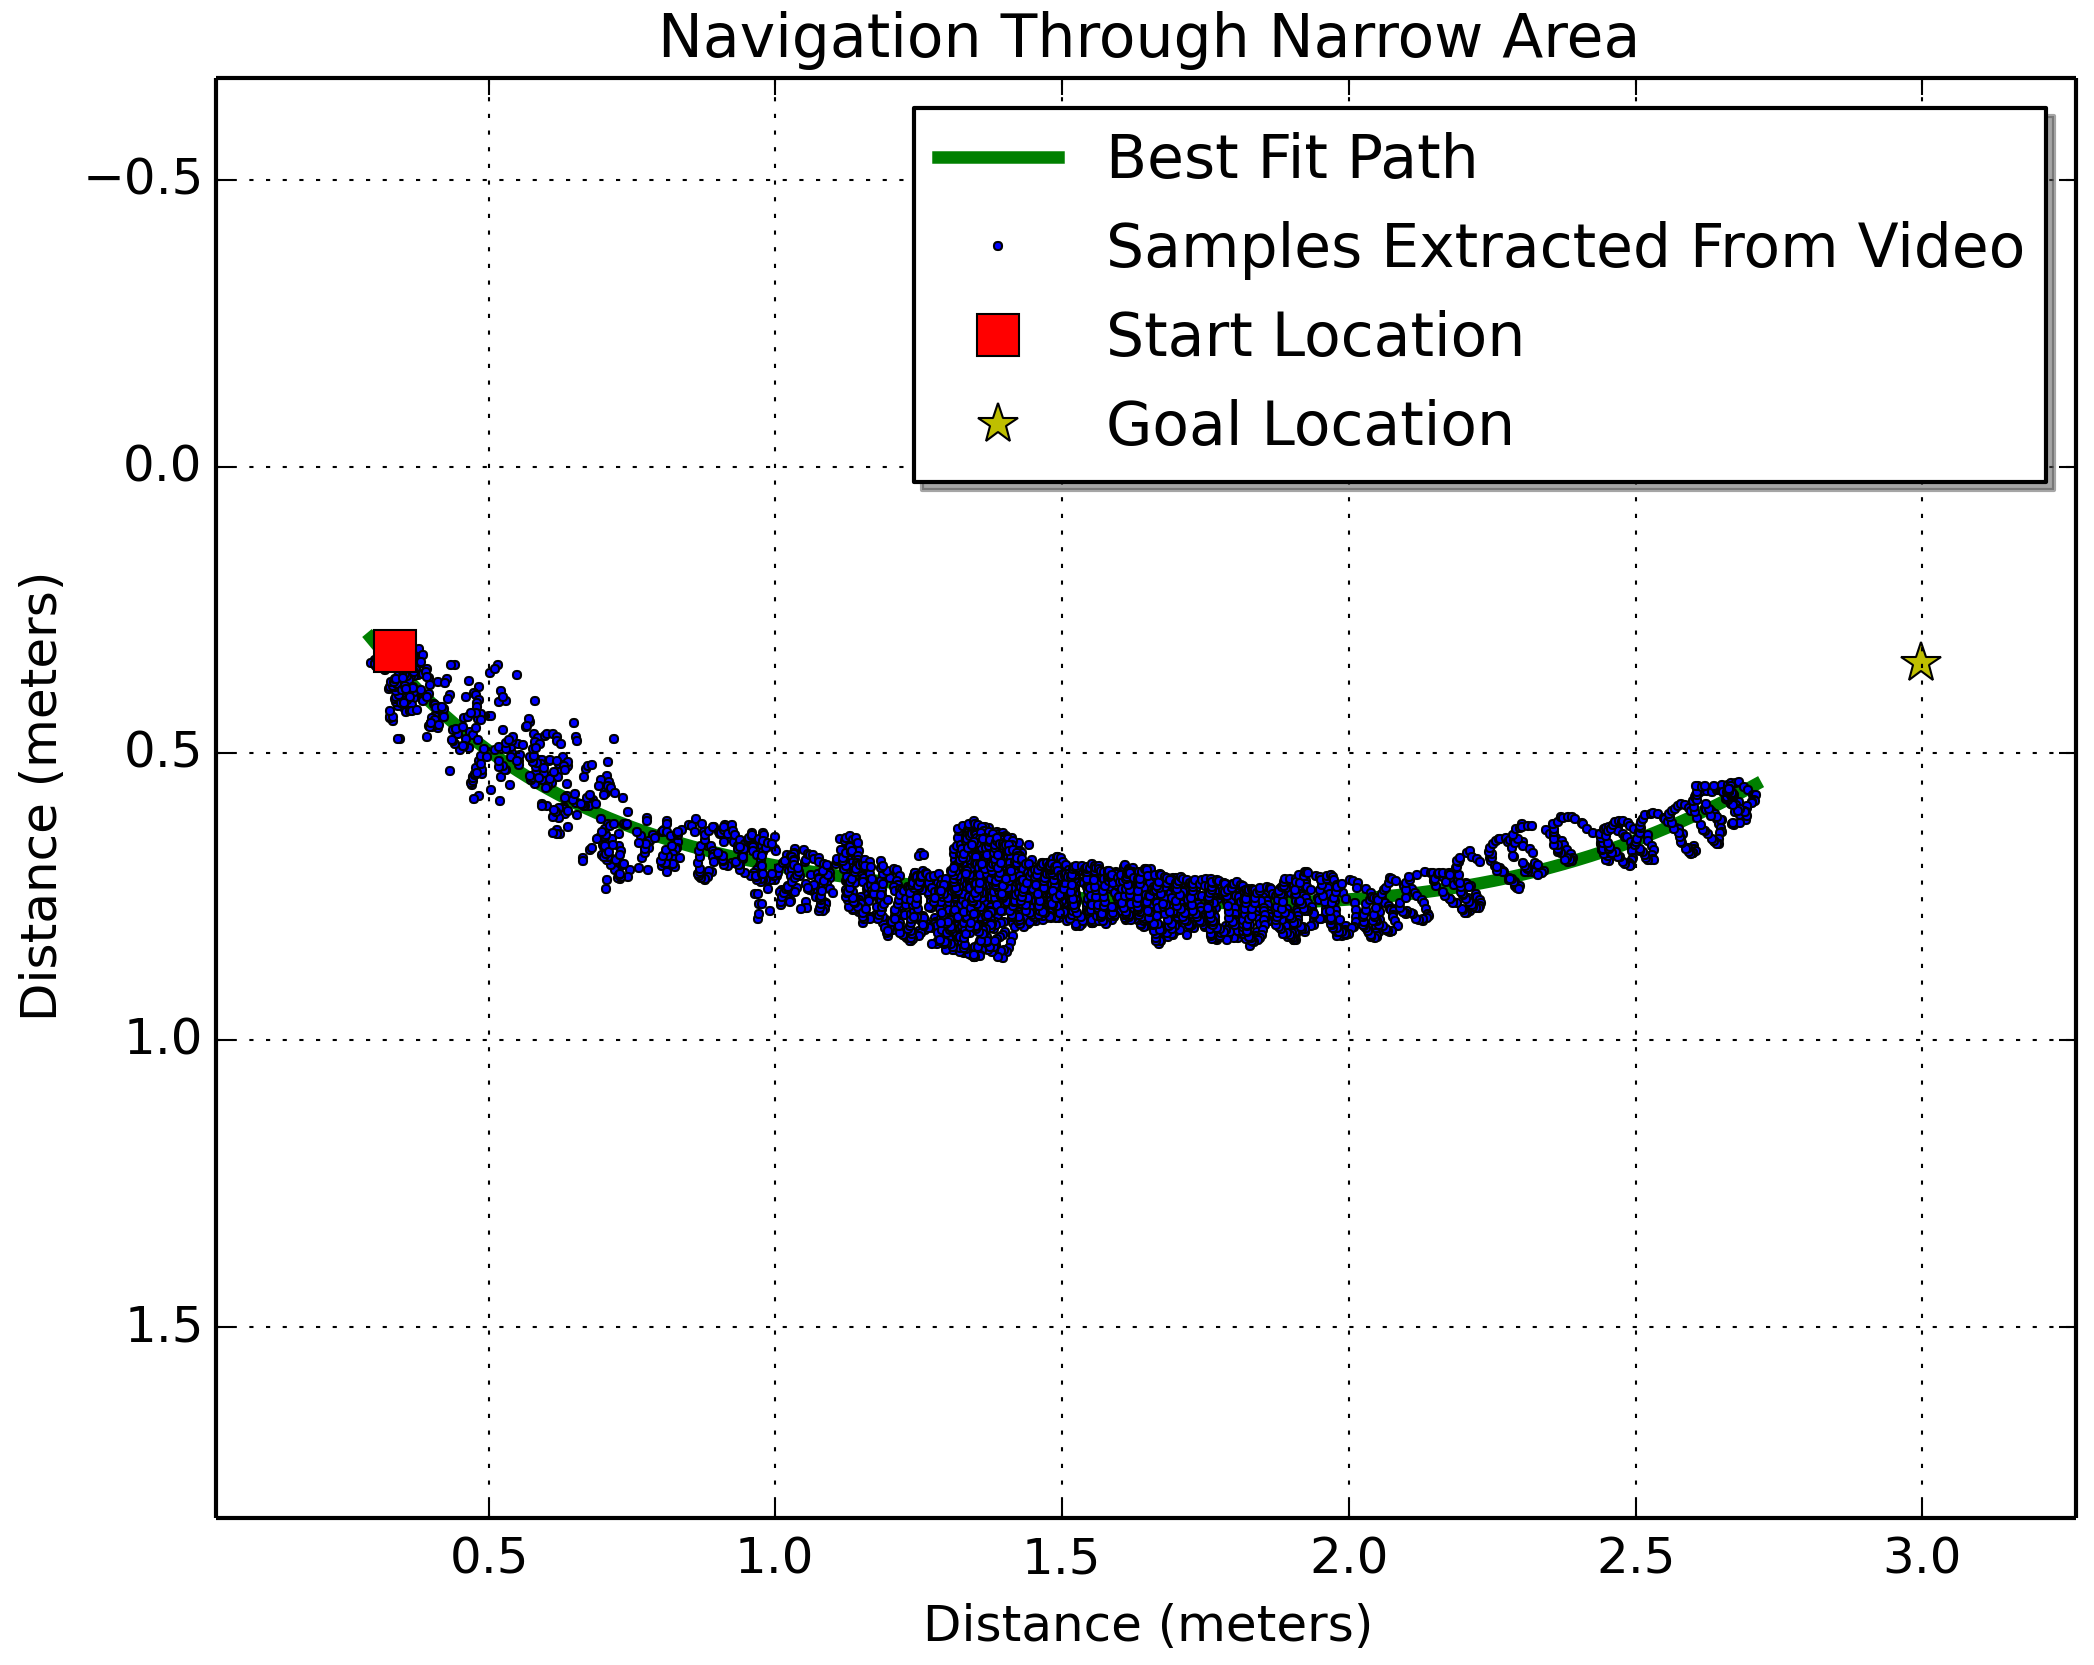
\includegraphics[width=\textwidth]{nav/narrow/plots/nav_narrow.png}
  \caption{Low-profile crawling gait for accessing vertically constrained spaces such as under a table.}
  \label{fig:nav_narrow_plot1}
\end{figure}

\begin{figure}
  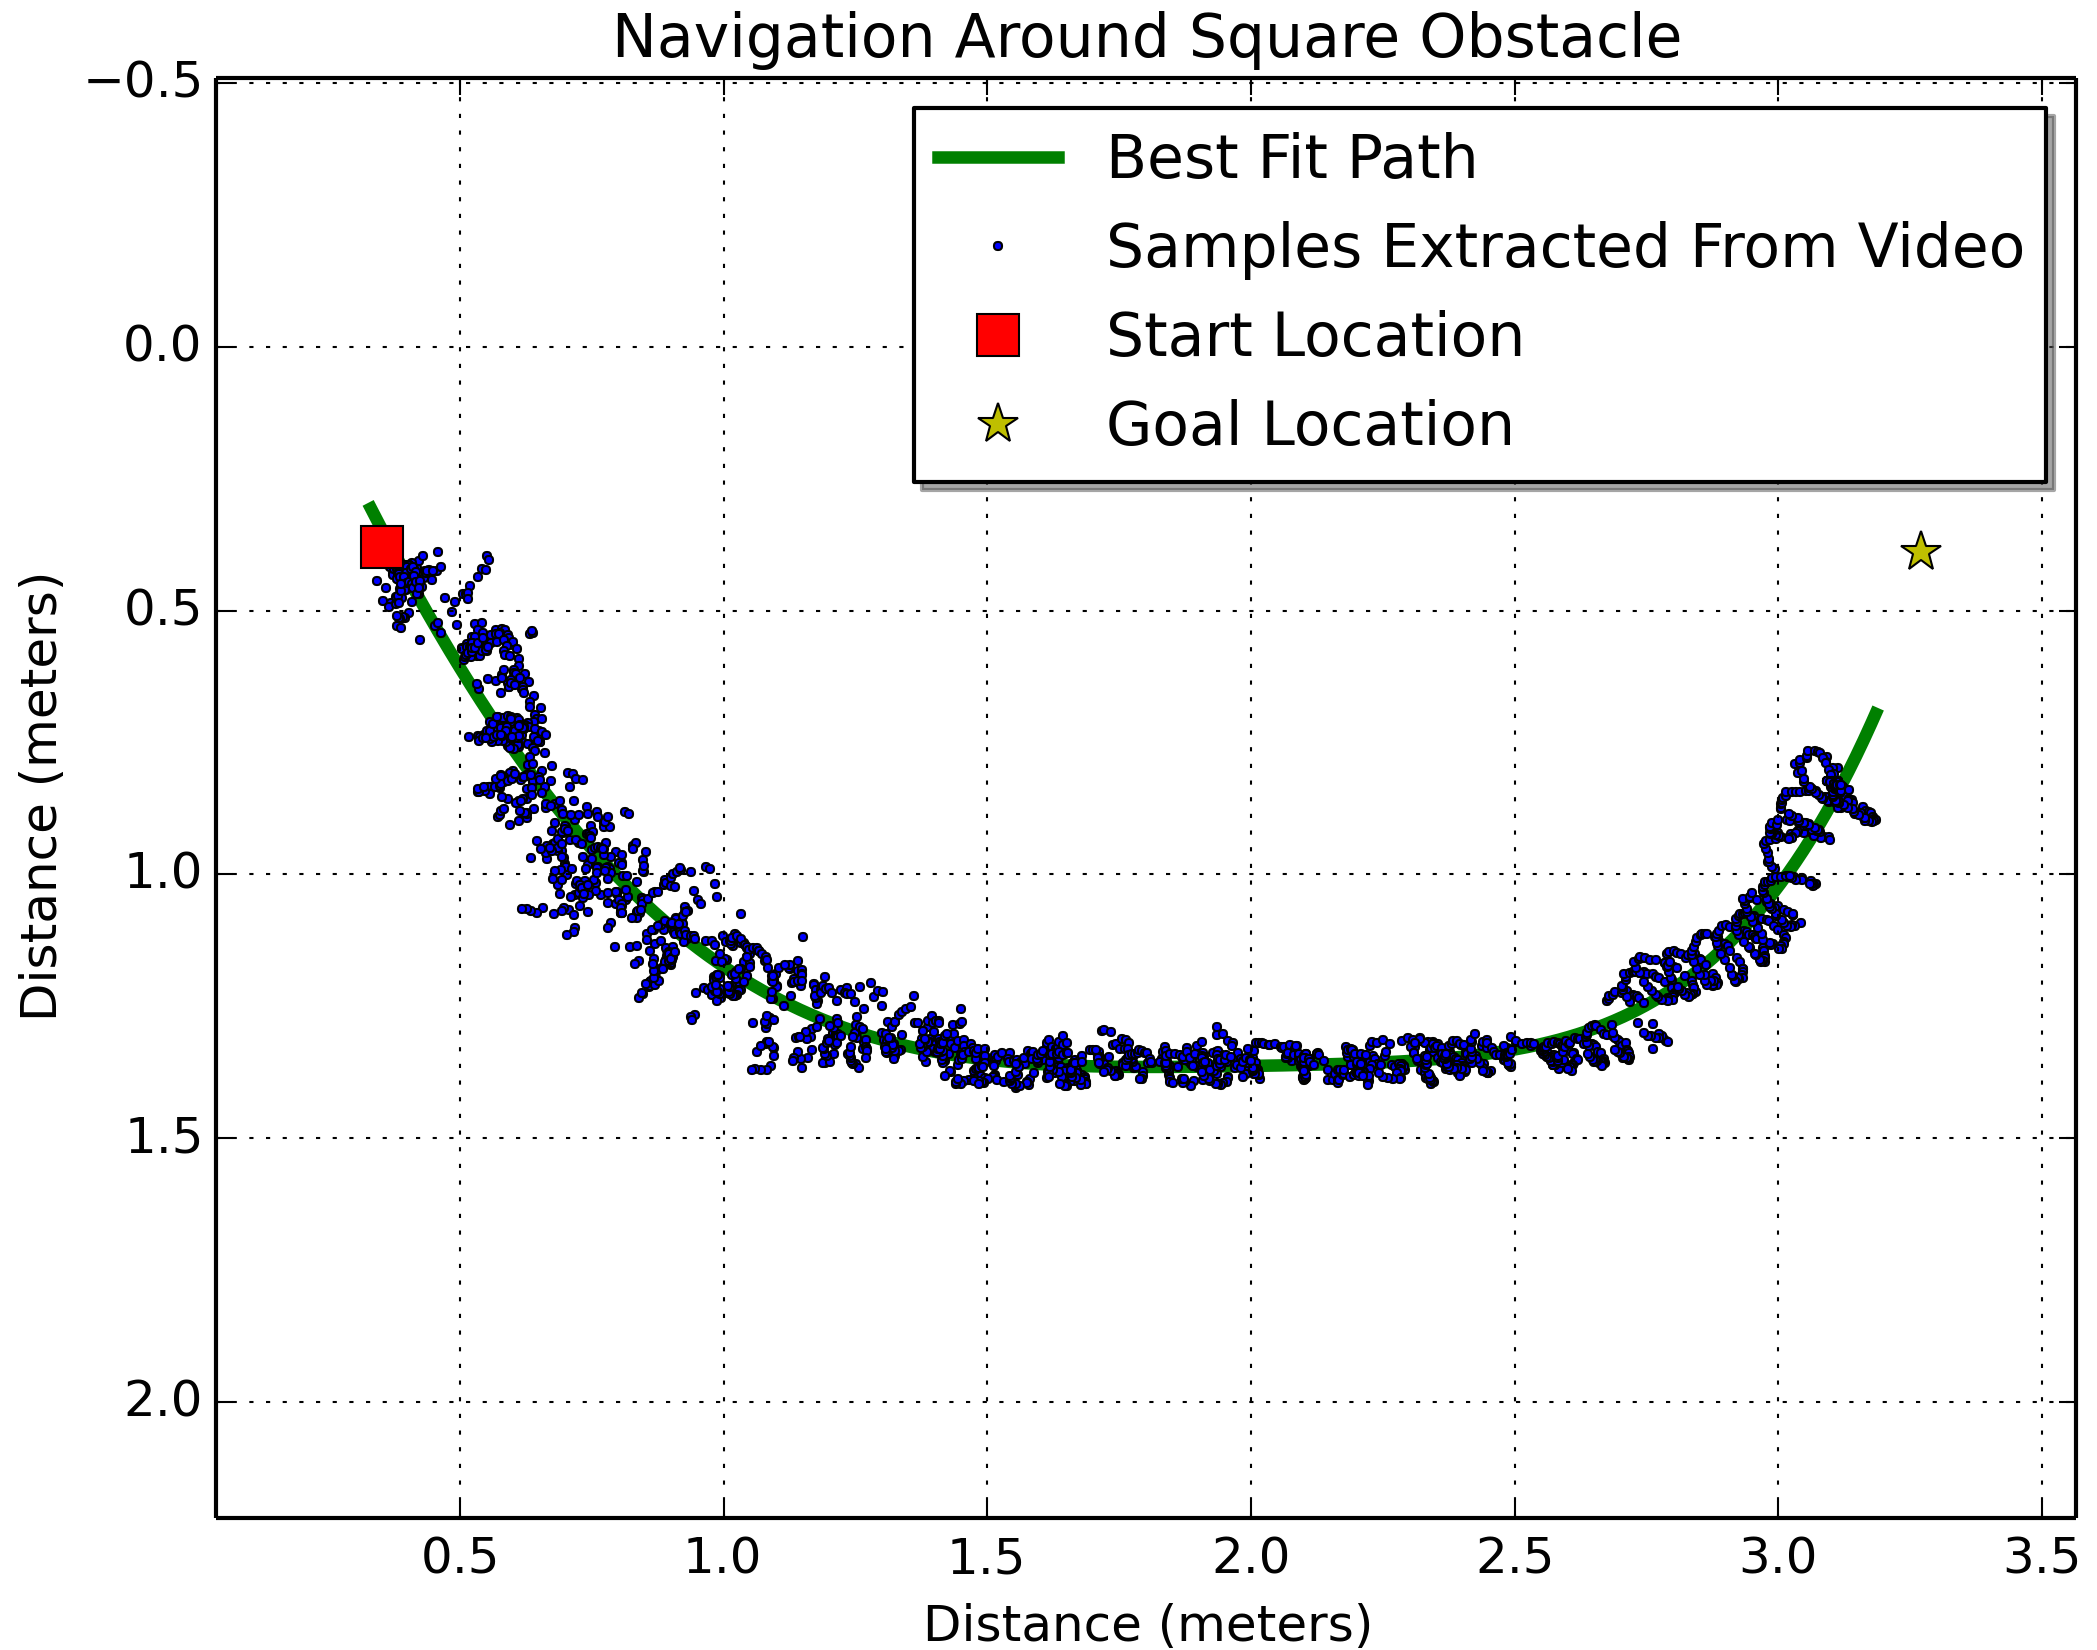
\includegraphics[width=\textwidth]{nav/square/plots/nav_square.png}
  \caption{Low-profile crawling gait for accessing vertically constrained spaces such as under a table.}
  \label{fig:nav_square_plot1}
\end{figure}

\begin{figure}
  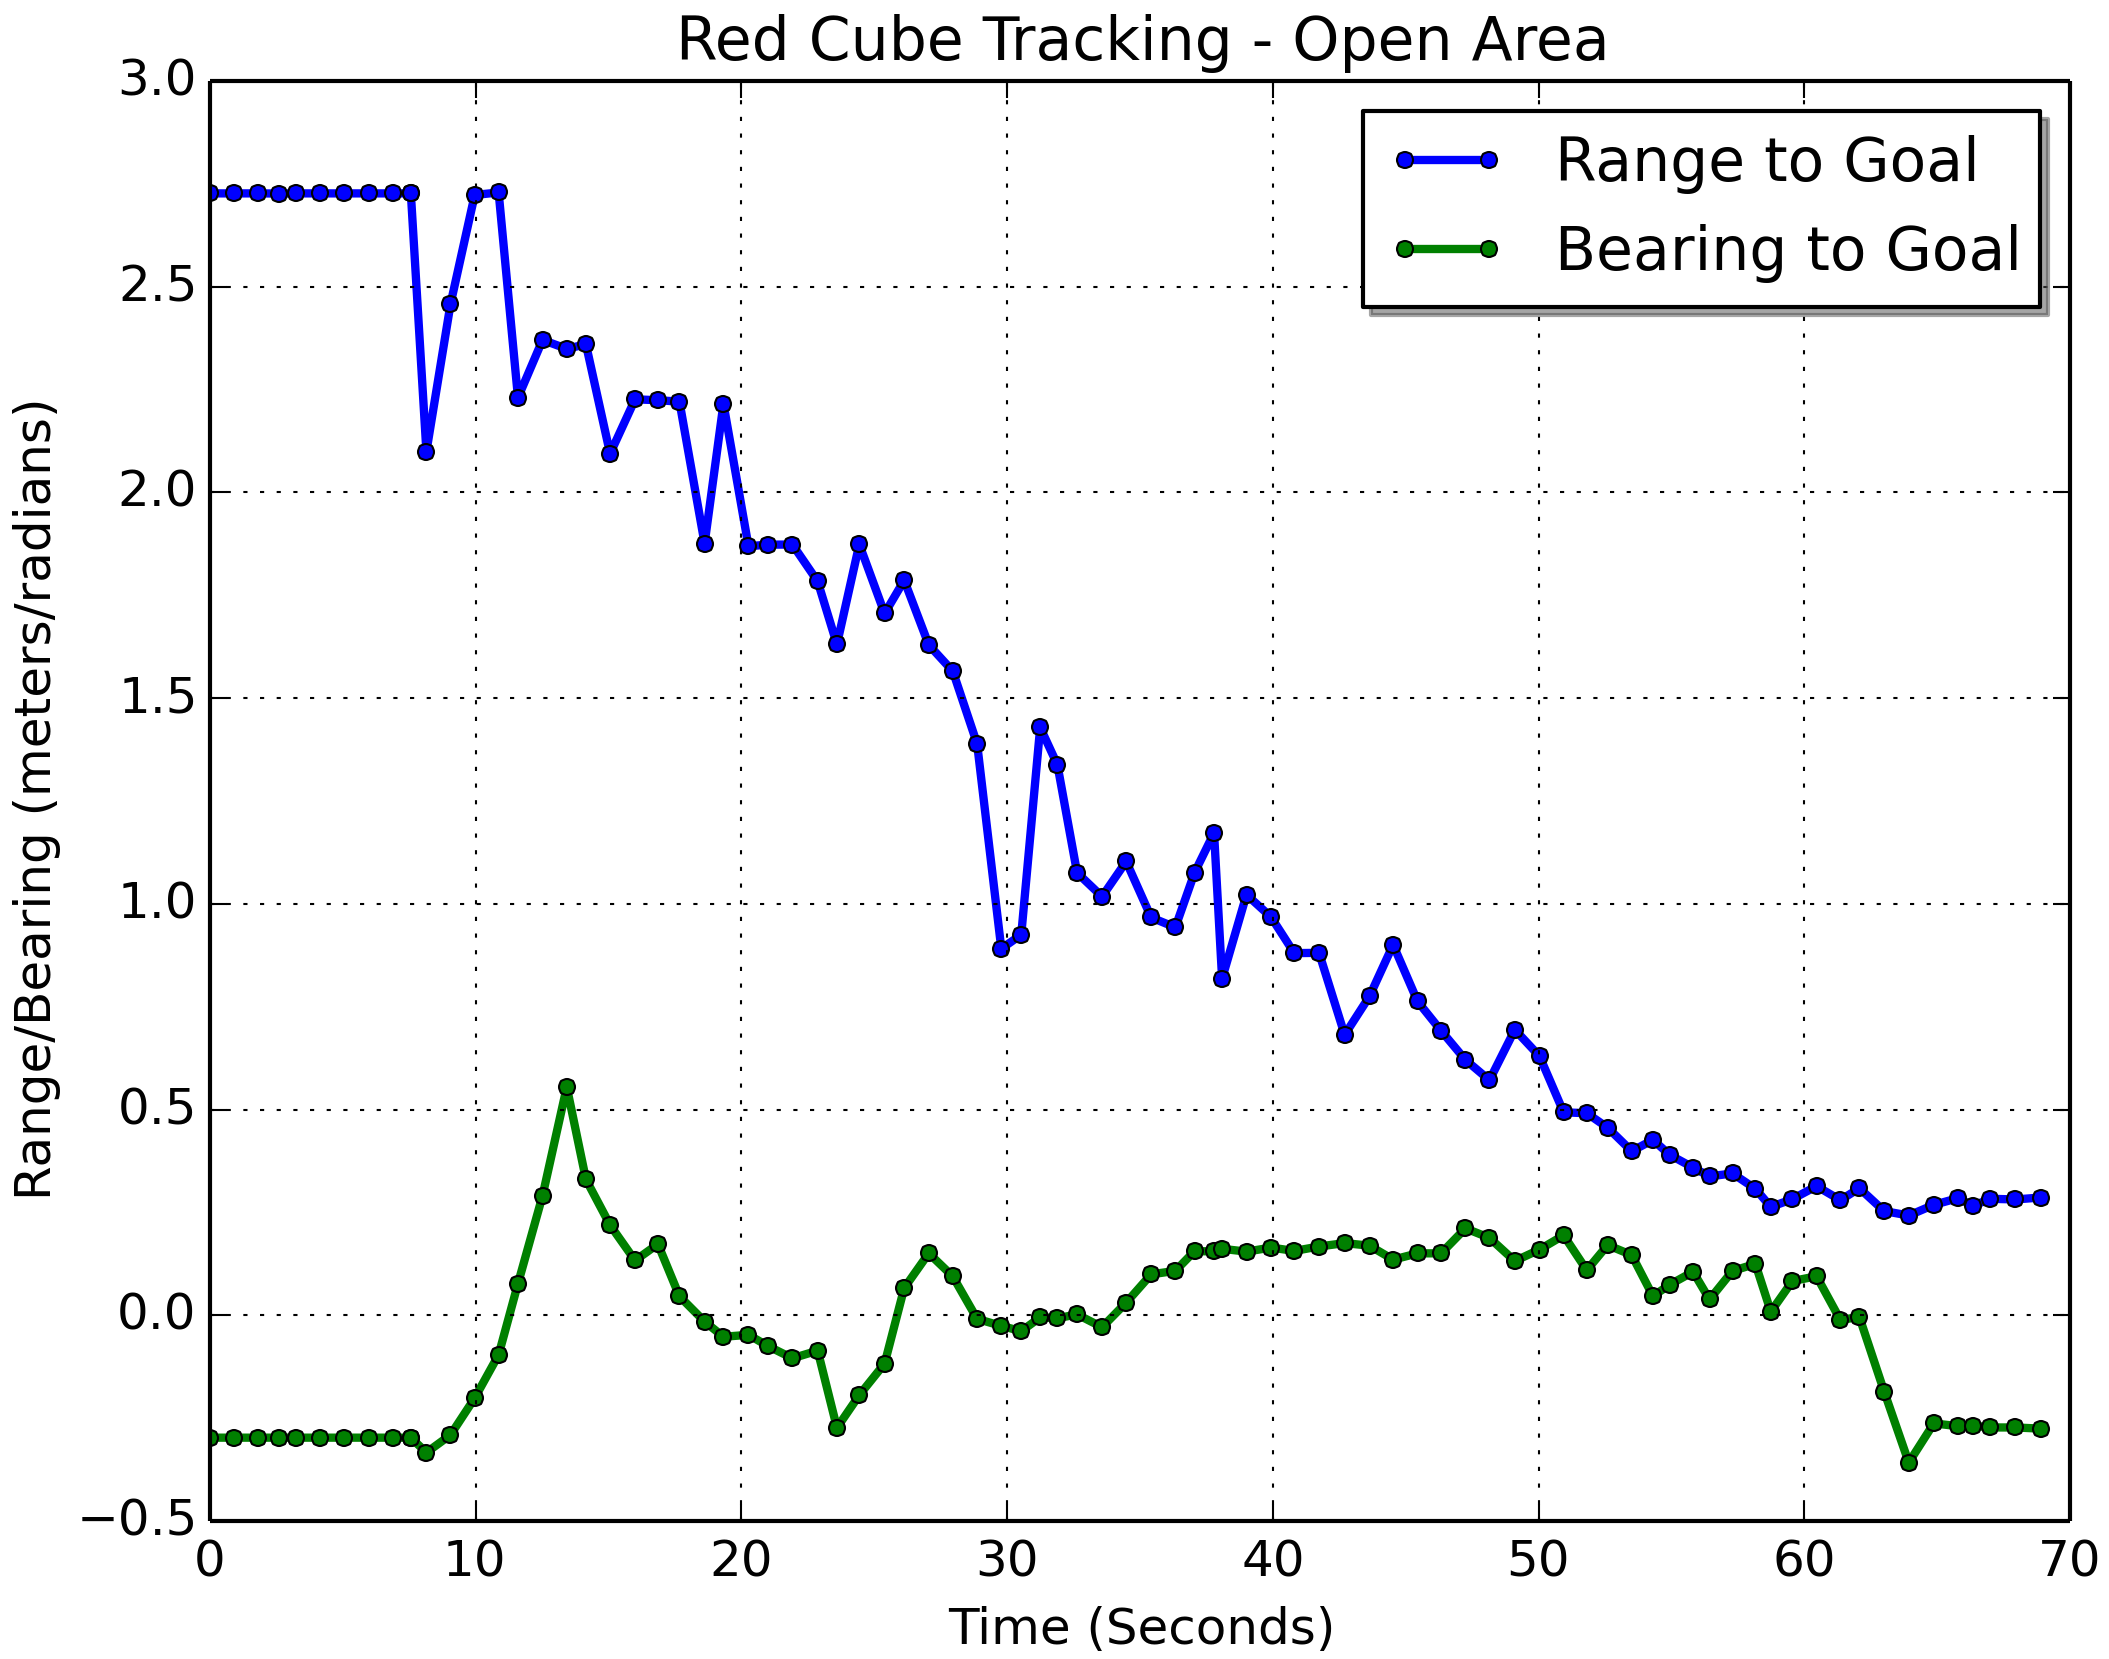
\includegraphics[width=\textwidth]{nav/open/tracking/open_rb1.png}
  \caption{Low-profile crawling gait for accessing vertically constrained spaces such as under a table.}
  \label{fig:nav_open_rb1}
\end{figure}

\begin{figure}
  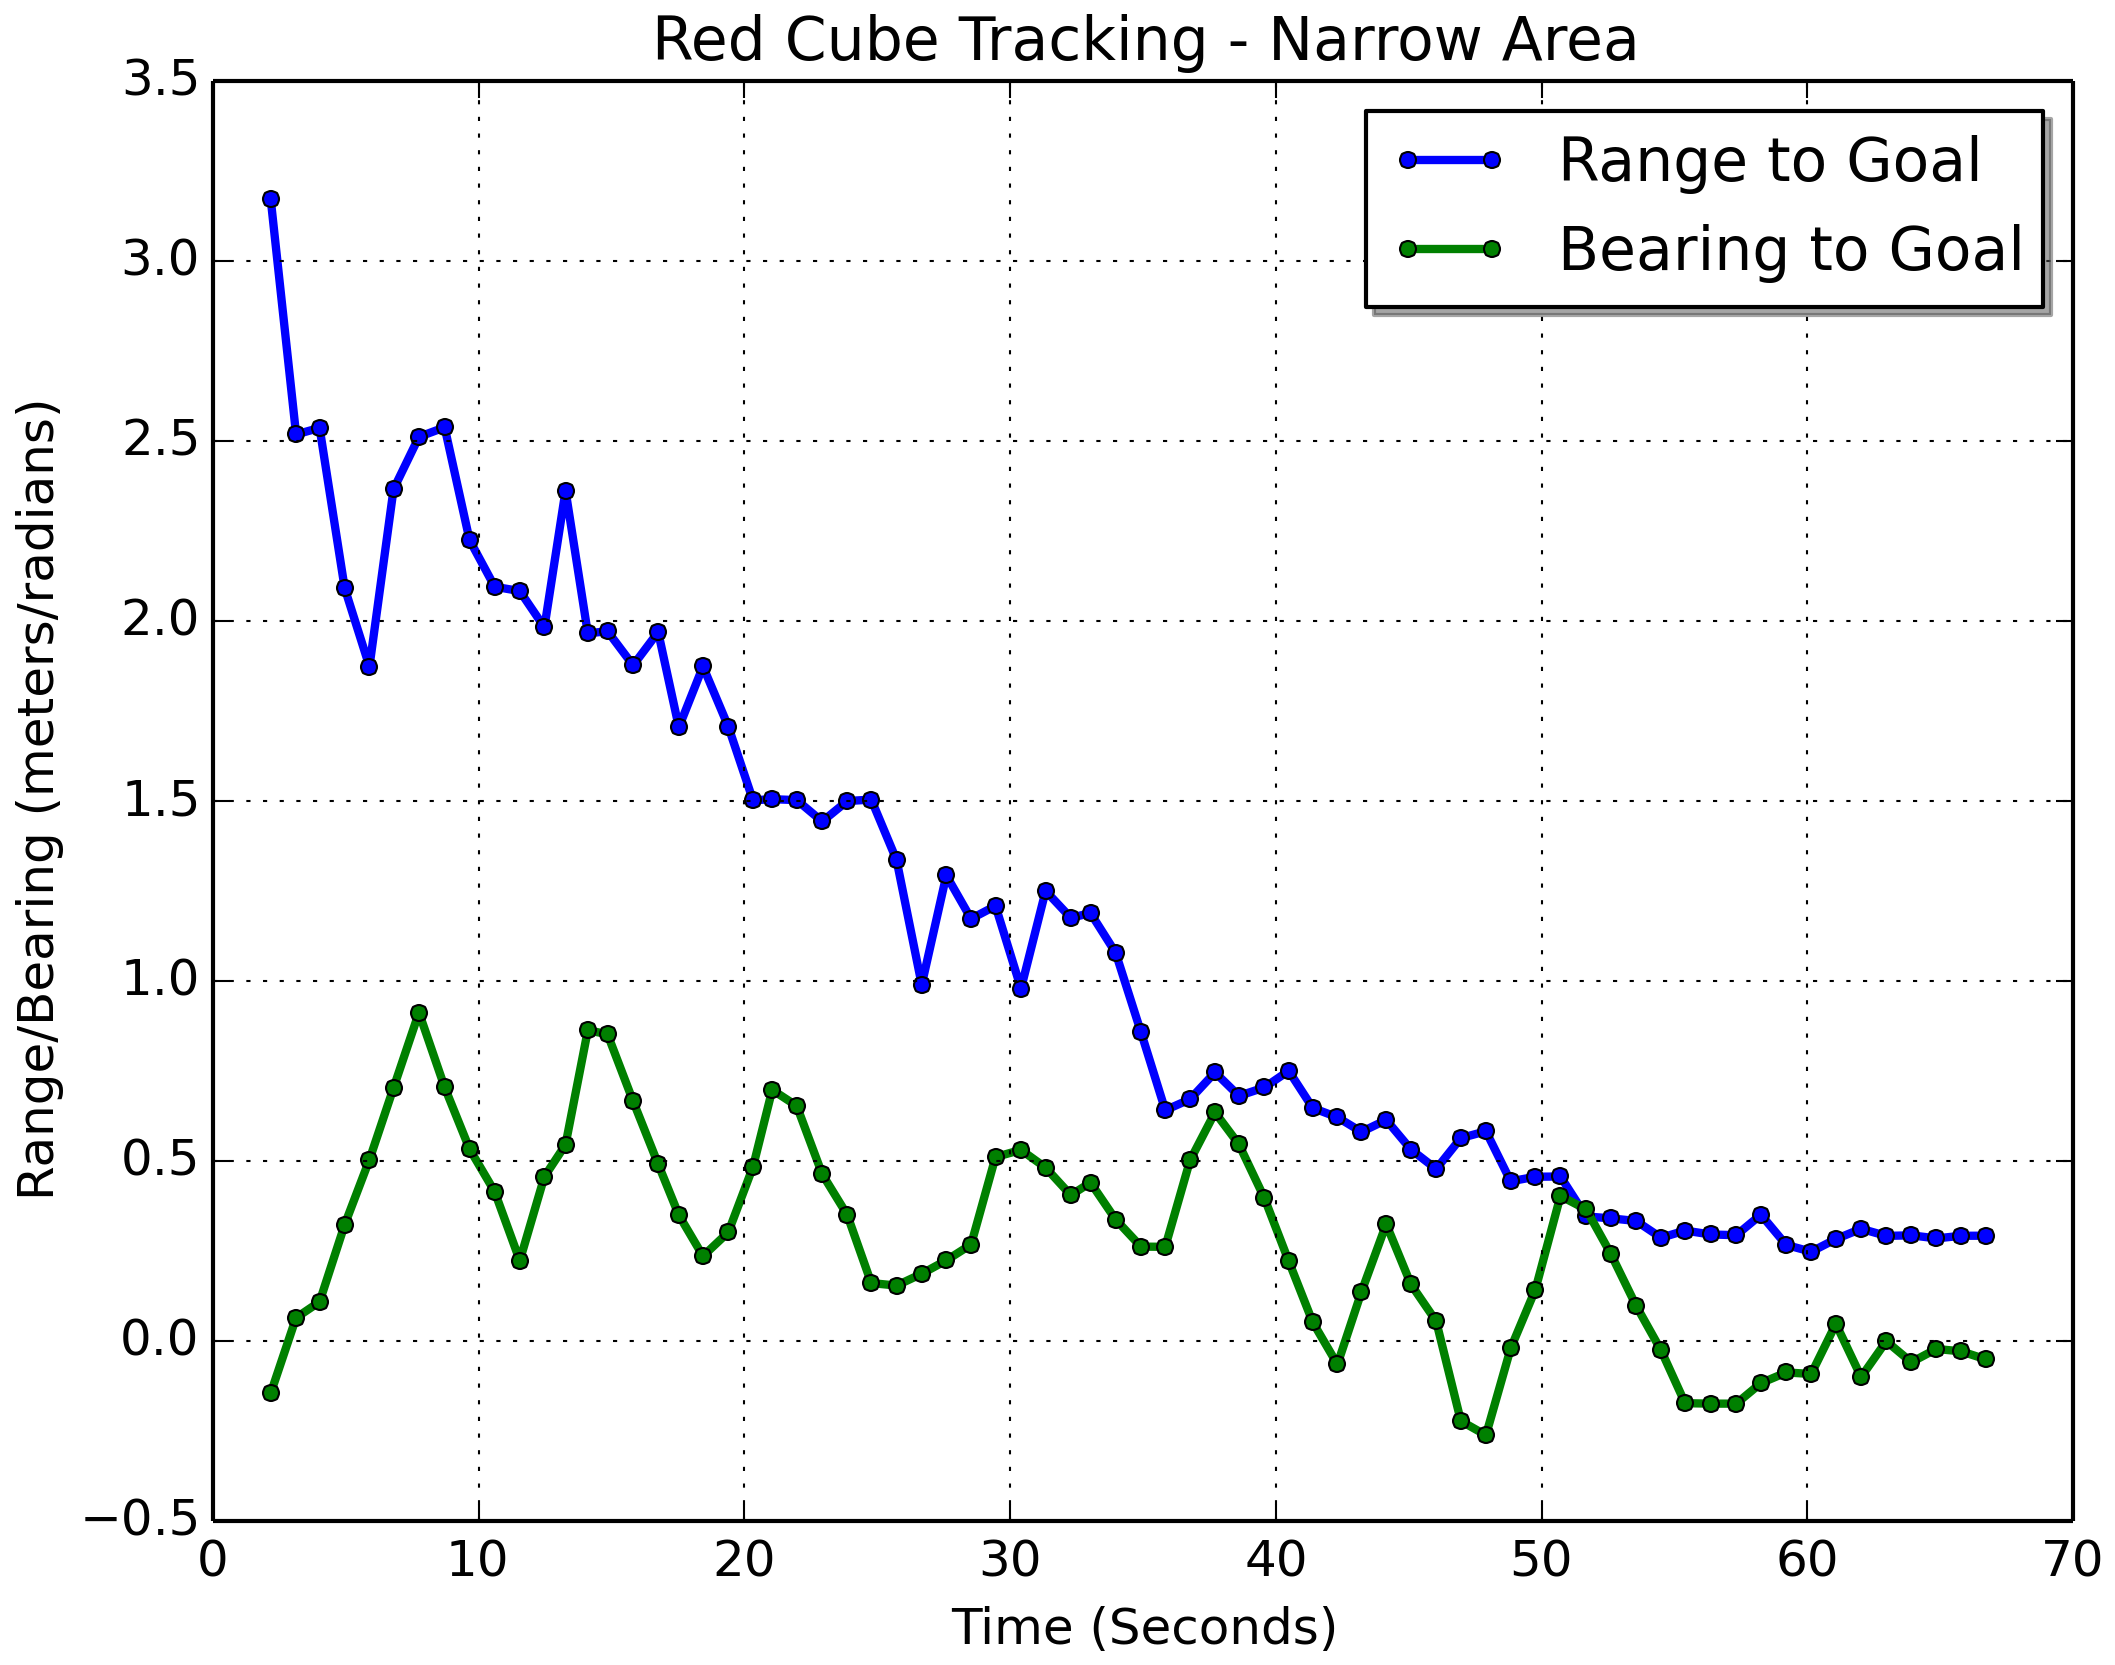
\includegraphics[width=\textwidth]{nav/narrow/tracking/narrow_rb1.png}
  \caption{Low-profile crawling gait for accessing vertically constrained spaces such as under a table.}
  \label{fig:nav_narrow_rb1}
\end{figure}

\begin{figure}
  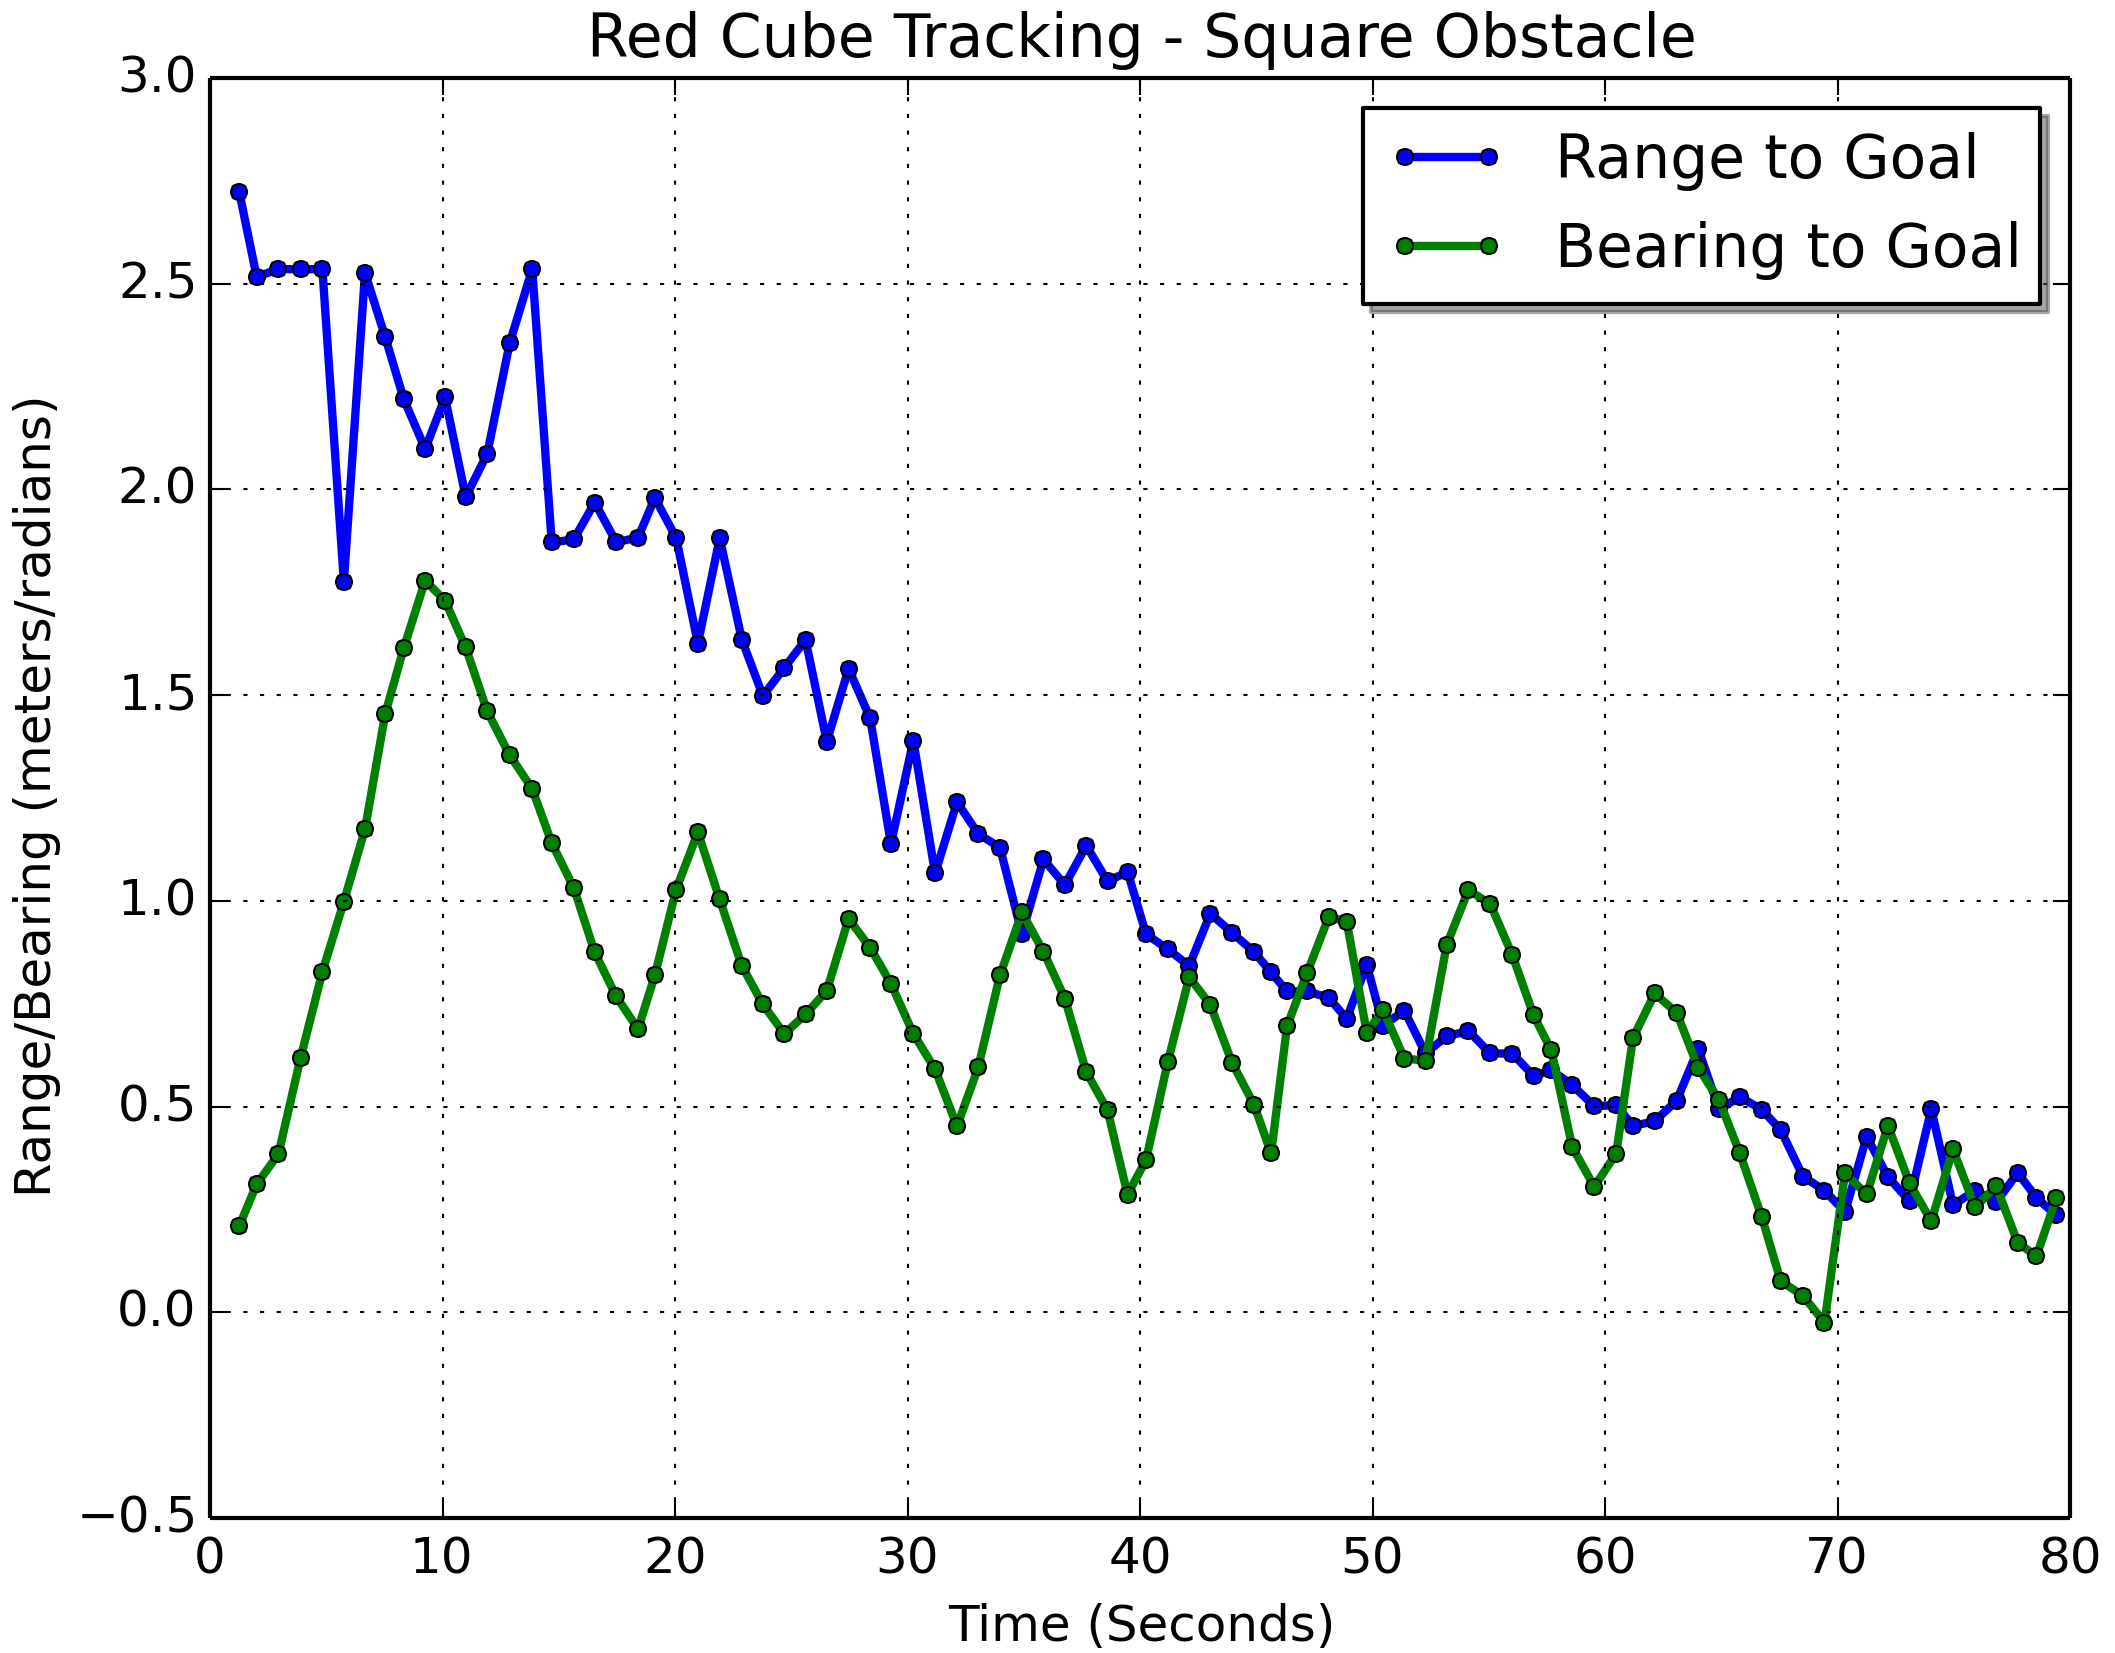
\includegraphics[width=\textwidth]{nav/square/tracking/square_rb1.png}
  \caption{Low-profile crawling gait for accessing vertically constrained spaces such as under a table.}
  \label{fig:nav_square_rb1}
\end{figure}